% !TeX root = ../main.tex
% Add the above to each chapter to make compiling the PDF easier in some editors.


% \chapter{Explainability of Fake News Detection Models}\label{chapter:explainability_of_fnd_models}
% AI is getting more and more integrated into our lives, helping us with from the simplest tasks like playing music with voice command to more complex tasks like driving a car in open traffic.
% \section{Explainability of News Content Models}
% \label{sec:explainabilityOfNewsContentModels}
% \subsection{SHAP, DeepSHAP}

% \subsection{SHAP in Action}

% \subsection{Introducing Unseen Data}

% \subsection{Results}

% \section{Explainability of Social Context Models}

% \subsection{GNNExplainer}

% \subsection{GNNExplainer in Action}

% \subsection{Introducing Unseen Data}

% \subsection{Results}

\chapter{Explaining Mixed Approaches for Fake News Detection}

\section{Mixed Approaches}
\label{sec:mixedApproaches}
As discussed in Section~\ref{sec:fakeNewsDetection}, social media's interconnected nature leads to fast dissemination of
fake news. When a news piece is shared, it cascades through social media by means of friendship networks. These networks
can be exploited to gather information about how fake news spread. Moreover, a user's historical information can prove effective when trying to analyze whether a news piece is real or not. This assumption stems from the psychological facts we discussed in Section~\ref{sec:fakeNewsDetection}. To recap, if a user is sharing fake news most of the time, i.e., the user's tweets are marked as fake, then it is likely that the next news piece they share would be fake as well. Usually, fake news are shared most within echo chambers, which gives rise to quick spread of fake news.\\
There exist many different approaches for social context models, however, it is a long and challenging task to create a dataset for social context models as the amount of data to be collected can grow dramatically. Thus, we selected a dataset that provides us with the social context information as well as the news content. Being a graph dataset, \emph{User Preference-aware Fake Detection} (UPFD)~\parencite{UPFD_Dataset_Shu} builds a propagation tree for the news. But in order to build a model that takes graphs as input we can no longer rely on standard deep learning approaches as the graph data has a different structure than news content data. It holds node information as well as edge information between nodes, allowing to store rich relational data~\parencite{UPFD_Dataset_Shu}.\\
In this section, we lay out foundations for the dataset and GNNs we used. Then we talk about the social context models along with their dataset UPFD that we used in this thesis. We also give some insights from~\parencite{HierarchicalPropagationNetworksForFND_Shu} in which the authors of UPFD dataset analyze the data they later utilized to create the graph dataset UPFD.\\

\subsection{Overview of Graphs}
\label{subsec:mixedApproaches_OverviewOfGraphs}
In this section, we introduce definitions to cover graphs and different types of GNNs. But we do not discuss each model type in detail due to GNNs' extensive background. Thus, we do not provide a notation for this section but we give mathematical definitions when required.\\
Graphs are an example of \emph{non-euclidean} data, meaning that in contrast to \emph{euclidean} data, they can represent complex relations and entities more accurate than one or two dimensional representations. Non-euclidean data used in GDL can be grouped into grids, graphs, groups, geosedics, and gauges, which are also called the 5G's of \emph{Geometric Deep Learning} (GDL)~\parencite{GeometricDeepLearning_Bronstein}. We are interested in one G only, graphs.
\begin{definition}[\emph{Geometric Deep Learning (GDL)}]
    A class of deep learning that aims to build models that can learn to predict on the non-euclidean domain.
\end{definition}
GDL is an extensive field covering various techniques that can be appied to non-euclidean domain. Due to its complex nature, we do not provide a rigorous background on GDL. For a detailed background on GDL, we refer the reader to an extensive study on GDL~\parencite{GeometricDeepLearning_Bronstein}. We only discuss parts related to GNNs that we utilized. First we define a graph.
\begin{definition}[\emph{Graph}]
    A graph is a non-euclidean type of data that represents the relations between entities.
\end{definition}
From the perspective of individual node connections, graphs can be categorized into two classes, \emph{directed} and \emph{undirected} graphs. Directed graphs have direction information in their edges, i.e., the information flows strictly from one node to another. On the other hand, undirected graphs do not have this limitation, the information flow is bidirectional. Since we are only interested in undirected graphs like our dataset, we give preliminaries for an undirected graph.\\
Following common notation on graphs, we define an undirected graph as $\mathcal{G} = (\mathcal{V}, \mathcal{E})$ with $\mathcal{V}$ as the set of nodes and $\mathcal{E}$ as the set of edges in a graph $\mathcal{G}$. We say that an edge $(v_i, v_j)$ exists between two nodes $v_i$ and $v_j$. Moreover, from the perspective of a graph's connectedness, there exist two types of graphs, \emph{cyclic} or \emph{acycylic}. Simply put, cyclic graphs have cycles in them, i.e., the graphs allows for at least one node $v_i$ to have a series of different edges that creates a cycle back to the node $v_i$. In contrast, acyclic graphs do not contain cycles. A concrete example for undirected acyclic graphs are trees. Also the structure of our dataset, trees have strictly one edge between two nodes.\\
When we look at graphs from node and edge type, we classify graphs as \emph{homogeneous} and \emph{heterogeneous} graphs. Homogeneous graphs have nodes and edges of the same type, whereas heterogeneous graphs have different types of nodes and edges. One example for homogeneous graphs are social networks in which the nodes are users and the edges represent the friendship between two users. If we modify this social network into a more detailed version in which we choose to represent another relationship between users, such as colleagueship, then we would have a heterogeneous graph, because there would be two types of edges in the graph.\\
Finally, if we consider graphs from a temporal aspect, we observe two kinds of graphs, \emph{static} and \emph{dynamic}. Static graphs stay the same over time, their topology or features do not change. In contrast, dynamic graphs' features and topology vary  over time, thus making time an important factor when working with dynamic graphs.

\subsection{Graph Neural Networks}
\label{subsec:mixedApproaches_GraphNeuralNetworks}
GNNs are neural networks that can take graphs as an input and produce predictions at three different levels:
\emph{node-level}, \emph{edge-level}, and \emph{graph-level}. Node-level tasks include node classification, node
regression, node clustering. Node classification aims to categorize nodes into classes. Node regression deals with
predicting continuous value for each node. Lastly, node clustering aims to group nodes into several clusters. Edge-level tasks consist of edge classification and link prediction. Edge classification tries to categorize an edge. Link prediction aims to find whether there is an edge between two nodes. Graph-level predictions are graph classification, graph regression, and graph matching. In all these settings, the model needs to learn representations of graph~\parencite{GNNsAReview_Zhou}.\\
In our experiments, we used two different models one of which uses a convolutional layer called GraphSAGE~\parencite{GraphSAGE_Hamilton} and the other uses a convolutional attention layer called \emph{Graph Attention} (GAT)~\parencite{GraphAttentionNetworks_Velickovic}. Here we give background for both but we do not dive into details. We first give information about general framework.\\
\cite{GNNsAReview_Zhou} defines three modules that are involved in a generic GNN model: \emph{propagation module}, \emph{sampling module}, \emph{pooling module}. Propagation module deals with information propagation between nodes so that the aggregated information can represent features and topology of the graph. Propagation modules usually employ a \emph{convolution operator} or \emph{recurrent operator} to aggregate information from neighbors of nodes separately. These aggregated values are then used to update the representation of the nodes, edges, and graph. Additionally these modules employ a skip connection that helps collect previous representations of nodes to alleviate the over-smoothing problem. Sampling module is used when the input graph is large to handle propagation. It is used before propagation module. Lastly, pooling modules are employed when we need to extract information to represent high-level graphs.\\
We will mostly deal with propagation module and the operations within. We do not dive into mathematical background of convolutions in detail but we introduce mathematical formulations in order to illustrate the operations our models are using. Also, we do not discuss recurrent operations on graphs as their background is extensive and out of scope of this thesis. We refer the reader to~\cite{GNNsAReview_Zhou} for an extensive mathematical baackground on convolutions and other operations on spectral domain. However, we will summarize the behavior of convolutions on graphs in order to give the sufficient knwoledge for the models we used.\\
\textbf{Convolutions on graphs.} The idea of convolution operators is to generalize convolutions from another domain to spectral domain. In general there are two types of convolutional operations.\\
The first, \emph{spectral approaches}, are based on graph signal processing and defines its convolutional operators in the spectral domain~\parencite{TheEmergingFieldOfSignalProcessingOnGraphs_Shuman}. Spectral methods initially transform a graph signal $x$ to the spectral domain by the graph Fourier transform $\mathcal{F}$, then the convolution operation is applied. The output from convolution is transformed back with the inverse Fourier transform $\mathcal{F}^{-1}$. Now we summarize the mathematics behind this approach in order to convey our models' characteristics. Graph Fourier and inverse graph Fourier transform are defined as,
\begin{center}
    $\mathcal{F}(x) = U^T x$
\end{center}
\begin{center}
    $\mathcal{F}^{-1}(x) = Ux$
\end{center}
where $U$ is the eigenvalue matrix of normalized graph Laplacian $L = I_N - D^{\frac{-1}{2}} A D^{\frac{-1}{2}}$ with $I_N$ the identity matrix of dimension $N$, $D$ as the degree matrix and $A$ as the adjacency matrix of the graph. $L$ is a real symmetric positive semi-definite matrix which helps us with factorization $L = U \Lambda U^T$ where $\Lambda$ denotes the diagonal eigenvalue matrix~\parencite{GNNsAReview_Zhou}. Now that we can convert our graph signal $x$ to spectral domain and back, following~\cite{AWaveletTourOfSignalProcessing_Mallat} and~\cite{GNNsAReview_Zhou}, we can define the convolution operation on $x$.
\begin{center}
    $g \star x = \mathcal{F}^{-1}(\mathcal{F}(g) \bigodot \mathcal{F}(x))$ \\ $= U(U^T g \bigodot U^T x)$
\end{center}
where $\bigodot$ stands for element-wise multiplication and $U^Tg$ is the convolution filter in the spectral domain. This can be further simplified into the basis function of spectral methods:
\begin{center}
    $g_w \star x = U g_w U^T x$
\end{center}
where $g_w$ is a diagonal learnable matrix. Essentially, all spectral methods use a convolutional filter $g_w$ but their choice of design creates a variety of approaches that are built upon each other. We only discuss the ones necessary for our models. The main idea of modern convolutional operators come from approximating $g_w$ with $k$-th order Chebsyshev polynomials. GCN adopts $k=1$ to avoid overfitting. Moreover, it introduces a renormalization trick to solve the exploding/vanishing gradient problem~\parencite{GCN_Kipf}. Further works like AGCN~\parencite{AGCN_Li} have employed a similar approach. Additionally, GCN is employed to an extent in spatial approaches.\\
The second, \emph{spatial approaches} focus on the graph structure. They define convolutions directly on graph topology. Spatial approaches can be grouped into \emph{basic}, \emph{attention-based}, and \emph{framework}. Basic spatial approaches define convolution operations on the neighborhoods of different sizes. Neighborhoods are defined based on nodes as follows $\mathcal{N}_v$ for a node $v$. There exist several basic spatial approaches such as the diffusion CNN (DCNN)~\parencite{DCNN_Atwood} which describes the neighborhhood for nodes using transition matrices, the learnable GCN (LGCN)~\parencite{LGCN_Gao} which utilizes CNNs as aggregators by applying max pooling on neighborhhood matrices.\\
Another example, GraphSAGE uses an inductive learning approach to sample then aggregate features from a node's local neighborhhood. GraphSAGE uniformly samples a fixed-size collection of neighbors then aggregates this collection to produce embeddings for the graph~\parencite{GraphSAGE_Hamilton}. More precisely, let us assume that we have learned the parameters of $K$ aggregator functions denoted as $\textsc{AGG}_k$, and a set of weight matrices $W^k$ where $\forall k \in \{1, \dots K\}$. $k$ can be referred to as layer or search depth. Then for each $k$ we go through all nodes $v \in \mathcal{V}$ and apply an aggregation then an update. Concretely, at each $k$ and at each $v$, let $h_v^{k-1}$ denote the hidden state of a node $v$ at layer $k-1$. Following the same notation, we refer to the hidden state of a node's neighborhood $\mathcal{N}_v$ at layer $k$ as $h_{\mathcal{N}_v}^k$. GraphSAGE formalizes its aggregation and update operation at layer $k$ as:
\begin{center}
    $h_{\mathcal{N}_v}^{k} = \textsc{AGG}_{k}(\{h_u^{k-1}, \forall u \in \mathcal{N}_v\})$
\end{center}
\begin{center}
    $h_v^k = \sigma(W^k [h_v^{k-1} || h_{\mathcal{N}_v}^k])$
\end{center}
where $||$ denotes concatenation of two vectors, $[h_v^{k-1} || h_{\mathcal{N}_v}^k]$ concatenated vector and $\sigma$
a non-linear activation function. GraphSAGE employs three different aggregators: \emph{mean aggregator}, \emph{LSTM aggregator}, and \emph{pooling aggregator}. Mean aggregator collects sampled neighborhood information and takes the element-wise mean of the vector set $\{h_u^{k-1}, \forall u \in \mathcal{N}_v\}$. The inductive version also includes previous layer representation of node $v$, $h_v^{k-1}$. LSTM aggregator uses an LSTM to collect neighborhood information. LSTMs are more expressive than mean aggregators. However, since LSTMs are not permutation invariant, i.e., they process
their inputs sequentially, they need a modification to work with unordered sets. Finally, pooling aggregator first independently feeds each neighbor's vector to a FCN, then apply a pooling operation on the output.\\
The third, \emph{attention-based approaches}, utilizes the same attention logic introduced in~\ref{subsec:newsContentModels_TransformerArch} by following~\cite{NeuralMachineTranslationByJointlyLearning_Bahdanau}. A recent work Graph Attention Networks (GAT)~\parencite{GraphAttentionNetworks_Velickovic} proposes to integrate attention into the propagation step by computing the hidden state for node $v$ at layer $k$ as follows:
\begin{center}
    $h_v^{k} = \sigma(\sum_{u \in \mathcal{N}_v} a_{vu} W h_u^k)$ \\
\end{center}
\begin{center}
    $\alpha_{vu} = \dfrac{exp(LeakyReLU(a^T[Wh_v || Wh_u]))}{\sum_{k \in \mathcal{N}_v}exp(LeakyReLU(a^T[W h_v || W h_k]))}$
\end{center}
with $W$ as the weight matrix, $a$ as the weight vector of feed forward network and the non-linear activation function LeakyReLU is defined as:
\begin{center}
    \[LeakyReLU(\gamma, x) =
        \begin{cases}
            x,          & if x \geq 0 \\
            \gamma * x, & otherwise   \\
        \end{cases}
    \]
\end{center}
The authors in~\cite{GraphAttentionNetworks_Velickovic} also utilize Multi-Head Attention in order to stabilize the
learning process of attention(also called self-attention or intra-attention)~\parencite{AttentionIsAllYouNeed_Vaswani}. Concretely, same as GraphSAGE defined $K$ aggregators, GAT defines $T$ independent attention heads to compute hidden states and then features of these hidden states are either concatenated,
\begin{center}
    $h_v^k = ||_{t=1}^T \sigma(\sum \alpha_{vu}^t W_t h_u^k)$
\end{center}
or averaged,
\begin{center}
    $h_v^k = \sigma(\frac{1}{T} \sum_{t=1}^T \sum_{u \in \mathcal{N}_v} \alpha_{vu}^t W_t h_u^k)$
\end{center}
to obtain the output where $\alpha_{vu}^t$ represents the normalized attention values of the attention head $t$.\\
The last convolutional spatial approaches cover general frameworks that aims to integrate multiple different models into one framework. A mixture model MoNet was proposed by~\cite{GeometricDeepLearningOnGraphsAndManifolds_Monti} which is a spatial framework for unifying models such as GCN~\cite{GCN_Kipf}, ~\cite{GeodesicCNNsOnRiemannManifolds_Masci}, DCNN~\cite{DCNN_Atwood} and many more in non-euclidean domain.\\
One more thing we need to investigate is graph sampling in order to cover everything that was utilized in this thesis. GNN models suffer from an issue called \emph{neighbor explosion} which stems from having massive sizes of supporting neighbors from all previous layers as the number of layers increases~\cite{GNNsAReview_Zhou}. Likewise, as graph size increases, we will encounter the same problem. Sampling is used to solve this issue and it can be done on three levels: \emph{node sampling}, \emph{layer sampling}, and \emph{subgraph sampling}. Node sampling creates a subset using the neighborhood set $\mathcal{N}_v$ of the node's $v$. As discussed previously, GraphSAGE~\parencite{GraphSAGE_Hamilton} employs node sampling. Layer sampling takes a different approach and it selects a subset of nodes for aggregation. Lastly, subgraph sampling deals with the graph as a whole. One approach is to use clustering algorithms to obtain these subgraphs~\parencite{ClusterGCN_Chiang}. Another is to sample nodes and edges from graph to create a subgraph~\parencite{GraphSAINT_Zeng}.\\

\subsection{Dataset and Models}
\label{subsec:mixedApproaches_DatasetAndModel}
Our choice of dataset, UPFD~\parencite{UPFD_Dataset_Shu} utilizes the dataset FakeNewsNet~\parencite{FakeNewsNet_Shu}. From FakeNewsNet, the authors of UPFD build a graph dataset by collecting user preference information from historical posts and social context data with Twitter Developer API~\parencite{TwitterAPI_Twitter}. They further employ textual embedding techniques to encode historical posts and news content. We shall discuss how these operations are conducted in detail. UPFD has two three preparation levels which the authors coined as \emph{endogeneous preference encoding}, \emph{exogeneous context extraction}, and \emph{information fusion}. The framework is shown in Fig~\ref{fig:UPFD_Framework}\\
\begin{figure}
    \centering
    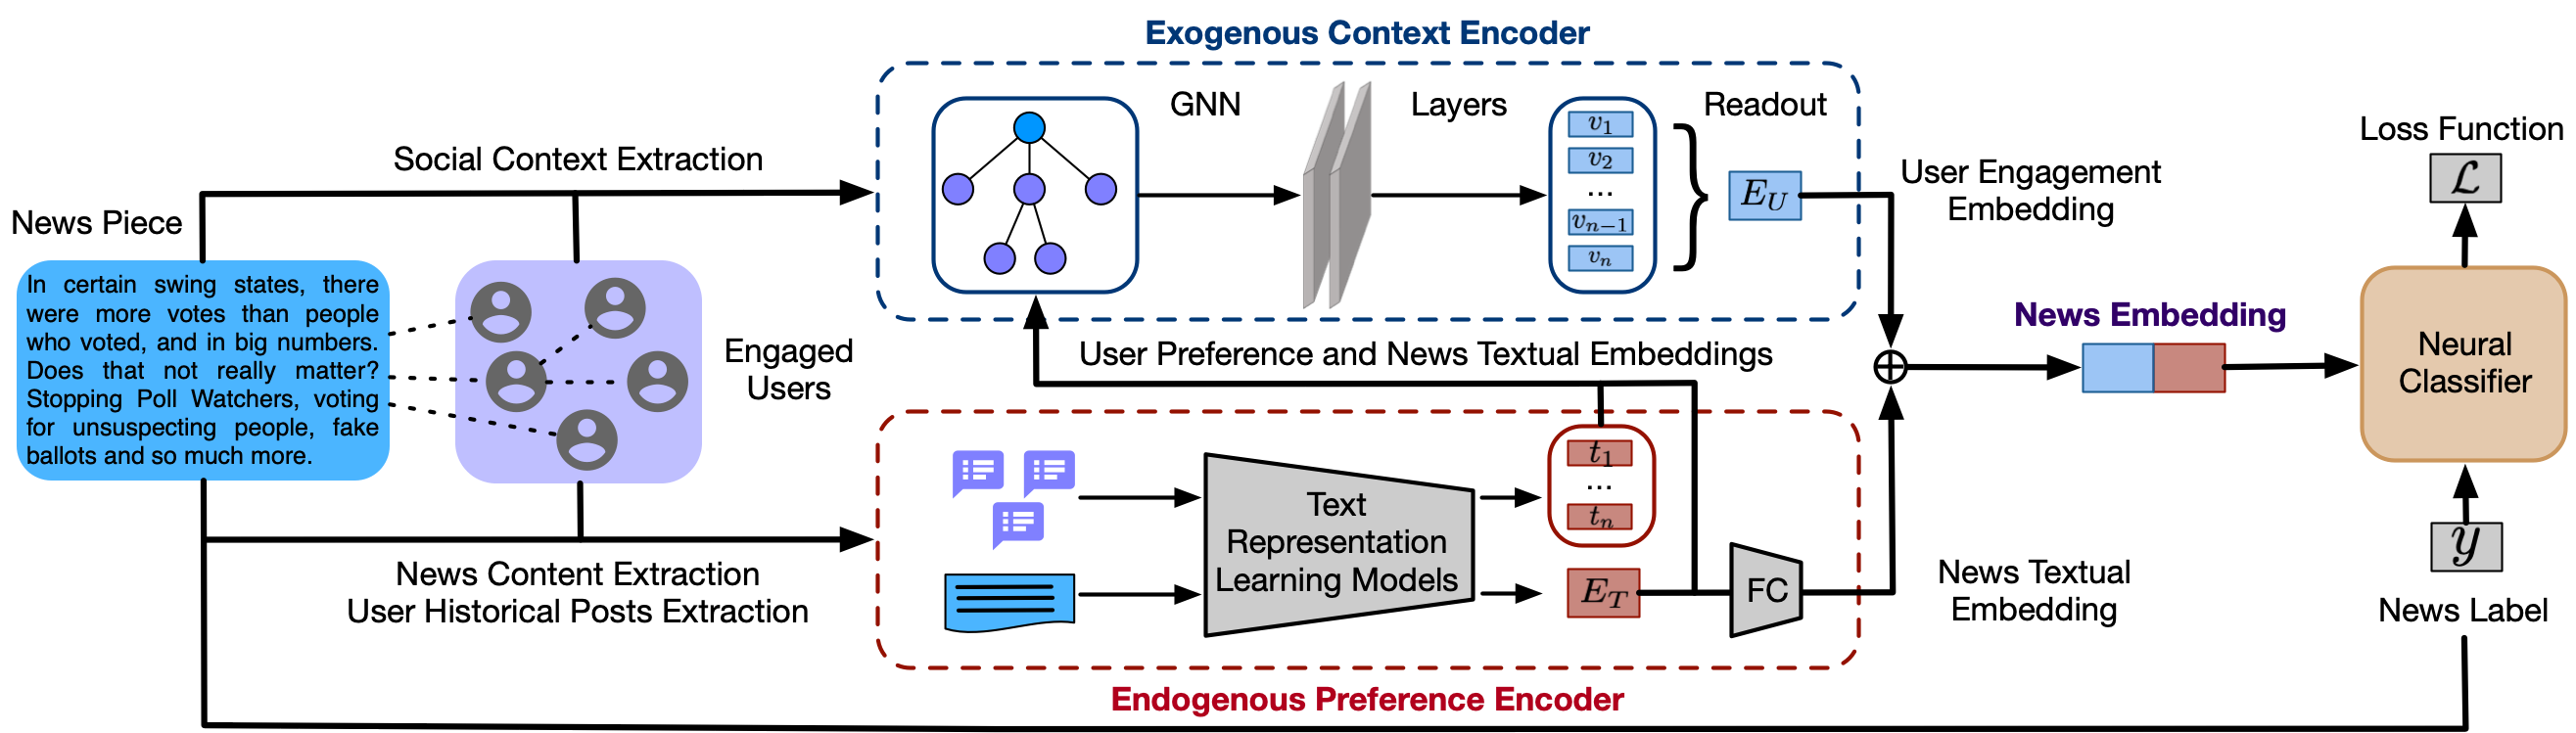
\includegraphics[scale=0.33]{UPFDFramework.png}
    \caption[UPFD Framework]{The framework of UPFD. Image obtained from~\parencite{UPFD_Dataset_Shu}}
    \label{fig:UPFD_Framework}
\end{figure}
\textbf{Endogeneous preference encoding} deals with user historical posts and news content using the news content and social engagement data in FakeNewsNet. With social engagement data, the authors collect 200 historical tweets of each user who have retweeted the news in FakeNewsNet. Summing up to almost 20 million tweets, these collection procedure of historical tweets for each FakeNewsNet news instance is as follows~\parencite{UPFD_Dataset_Shu}:
\begin{itemize}
    \item Collect user ids who have retweeted.
    \item For each user, collect 200 most recent tweets.
    \item For inaccessible (suspended or deleted) users, use randomly sampled tweets from accessible users who engage the same news piece. This step also increases the effectiveness of the exogeneous encoder.
    \item  Finally, remove special characters such as "@" and URLs before applying textual techniques.
\end{itemize}
Now that we have news content and user historical information, we encode these texts using text representation learning techniques. Still following~\cite{UPFD_Dataset_Shu}, the authors define two different settings for creating endogeneous preference encoding. The first setting, \emph{spacy}, deals with obtaining the representation for user historical data and news content with spaCy~\parencite{SpaCy_Honnibal} pretrained 300-dimensinal vectors for 680K words. For each user historical post (and similary for each news piece), if a word appears in the text, we include the vector for that word for final calculation in which all included vectors are averaged. As a result, we obtain a 300-dimensinal vector for each user historical information and news piece. The second setting, \emph{bert}, uses BERT-Large model to encode news and historical user data. Using bert-as-a-service~\parencite{BertAsAService_Xiao}, the authors encode the news content with maximum input sequence length as 768. To encode historical information, the authors opt for a different setting since 200 tweets cannot be processed as a single document due to BERT's maximum input sequence length limitation of 768. It is important to note that the paper of UPFD~\parencite{UPFD_Dataset_Shu} states the maximum input sequence length as 512, however in the dataset itself, the maximum sequence length is 768~\parencite{UPFD_PyGTeam}. Keeping in mind that tweets are usually short texts compared to news pieces, the authors use maximum input sequence length of 16 for each historical tweet, then average all 200 tweets to obtain the final representation for user historical data. This representation is of the same dimension as the root news node. Note that these text representation vectors are node features of a hierarchical tree structured graph whose root node represents the news content and the children of root represent the users who have retweeted.\\
\textbf{Exogeneous context extraction} uses retweet information to build the previously mentioned hierarchical tree. The authors adopt a similar procedure used in~\cite{GraphNeuralNetworksWithContinualLearningFakeNewsDetection_Han,GeometricDeepLearningOnGraphsAndManifolds_Monti,HierarchicalPropagationNetworksForFND_Shu}. In detail, authors define a news piece as $v_1$ and the set of users who retweeted $v_1$ as $\{v_2, \dots , v_n\}$ ordered by time. The rules are defined for this process to cover edge cases as well:
\begin{itemize}
    \item Estimate that a news piece propagates to user $v_i$ from user $v_j$ with the latest timestamp, if any user from the set $\{v_j | j\in \{2, \dots, n\}\setminus \{i\}\}$ retweeted the news piece before the user $v_i$. This conservative assumption is based on the fact that latest tweets are presented to the user first in the Twitter app~\parencite{UPFD_Dataset_Shu}.
    \item If user $v_i$ does not follow any users in the set $\{v_1, \dots, v_n \} \setminus {i}$, i.e., all retweeters and news source except the user itself, the authors approximate the spreader of that news piece to user $v_i$ as the user with most followers in the set. This approximation is based on the phenomena that the tweets from accounts with more followers have a higher probability of being retweeted or viewed.
\end{itemize}
After this procudure, we have our hierarchical tree for each news obtained from FakeNewsNet which employs two sources: Politifact and Gossipcop. Thus, we evaluate these datasets separately within UPFD. The distribution of the instances with respect to train/val/test split and label is provided in Fig.~\ref{fig:UPFD_Dataset_Visualization}.\\
\begin{figure}
    \subfloat[Gossipcop]{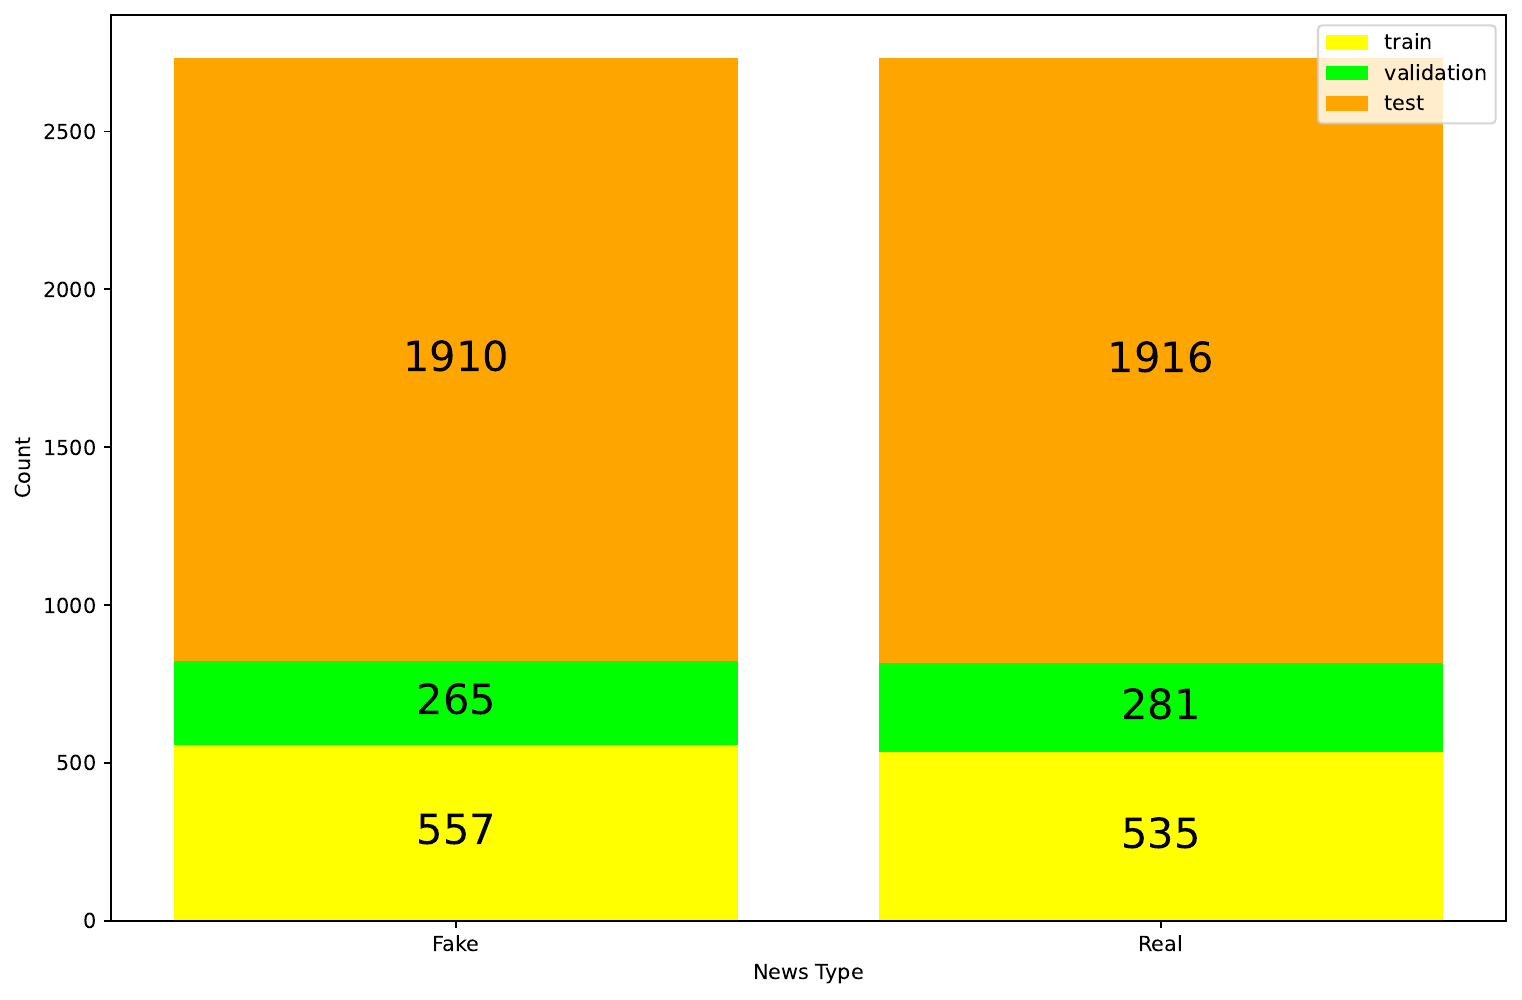
\includegraphics[width=0.45\textwidth]{GOS_DatasetDistrByLabelAndSplit.png}}
    \hfill
    \subfloat[Politifact]{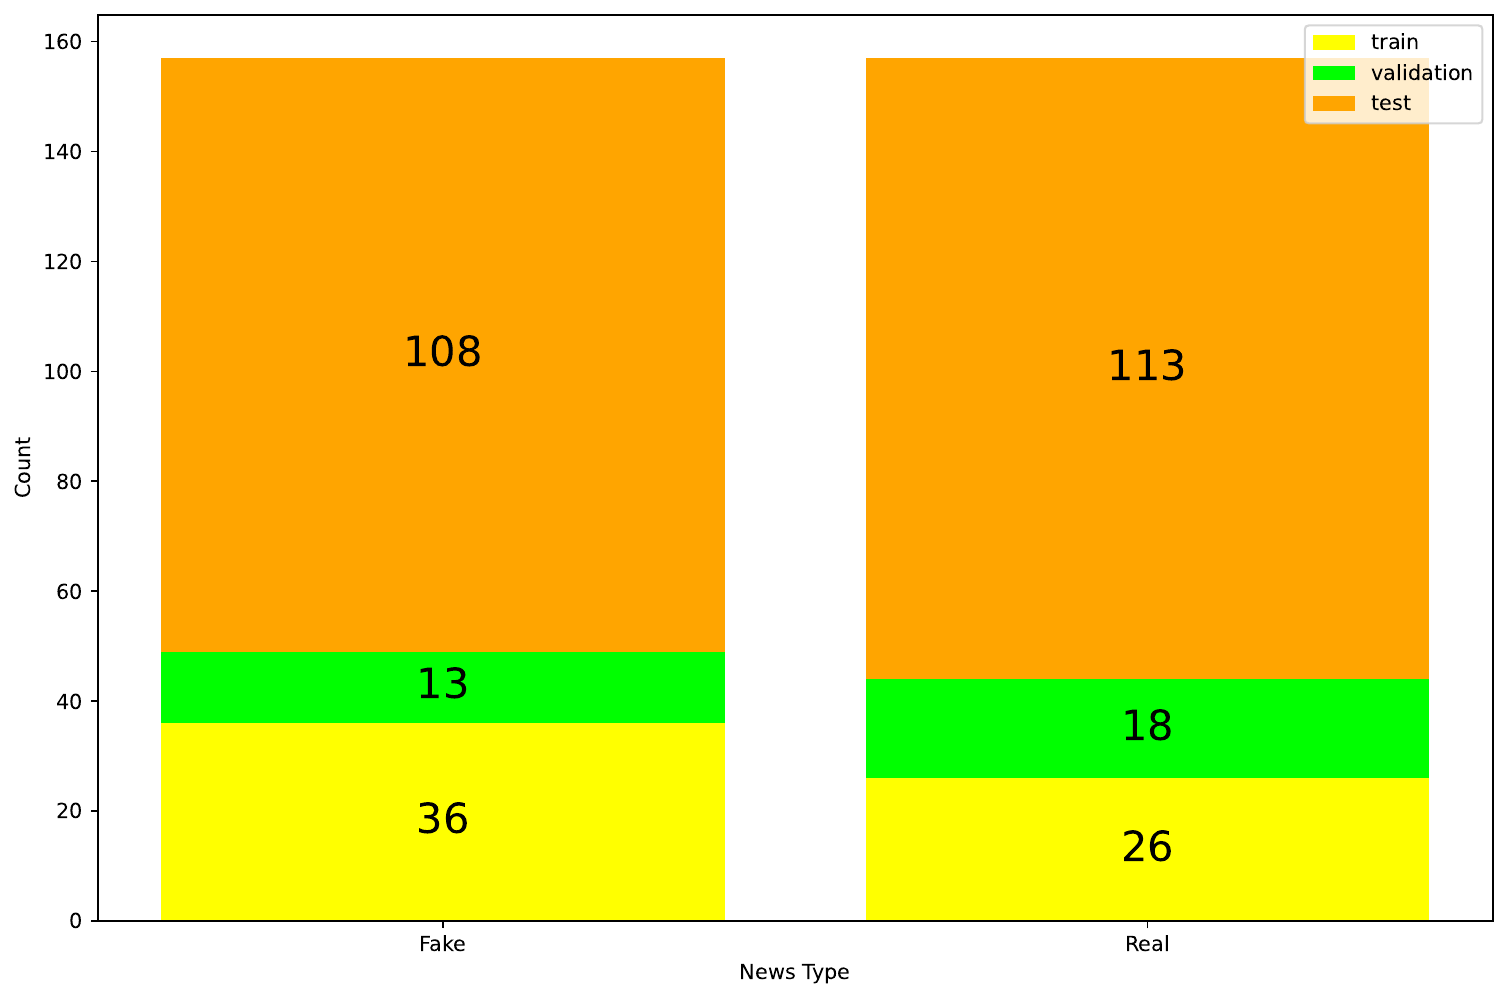
\includegraphics[width=0.45\textwidth]{POL_DatasetDistrByLabelAndSplit.png}}
    \caption[UPFD dataset distribution by label and split]{UPFD dataset distribution by label and split (train: 20\%, val: 10\%, test: 70\%)}
    \label{fig:UPFD_Dataset_Visualization}
\end{figure}
\textbf{Information fusion} is achieved via GNNs. As discussed in~\ref{subsec:mixedApproaches_GraphNeuralNetworks}, GNNs can encode graphs by maintaining the node features and structural information. From this point on, we need to utilize the models we introduced with a classification setting. Classification is done for each graph which represents the diffusion tree of the news piece~\parencite{UPFD_Dataset_Shu}. We adopted two models from this work's ablation study, the first one is based on GraphSAGE~\parencite{GraphSAGE_Hamilton}, and classification is handled with an FCN. We use BERT as the encoder since the best performance is obtained via that according to the experiments in~\cite{UPFD_Dataset_Shu} and the experiments we conducted. We call this model UPFD model as authors did in~\cite{UPFD_Dataset_Shu}. It is illustrated on Fig~\ref{fig:UPFDClassifierArchitecture}.
\begin{figure}
    \centering
    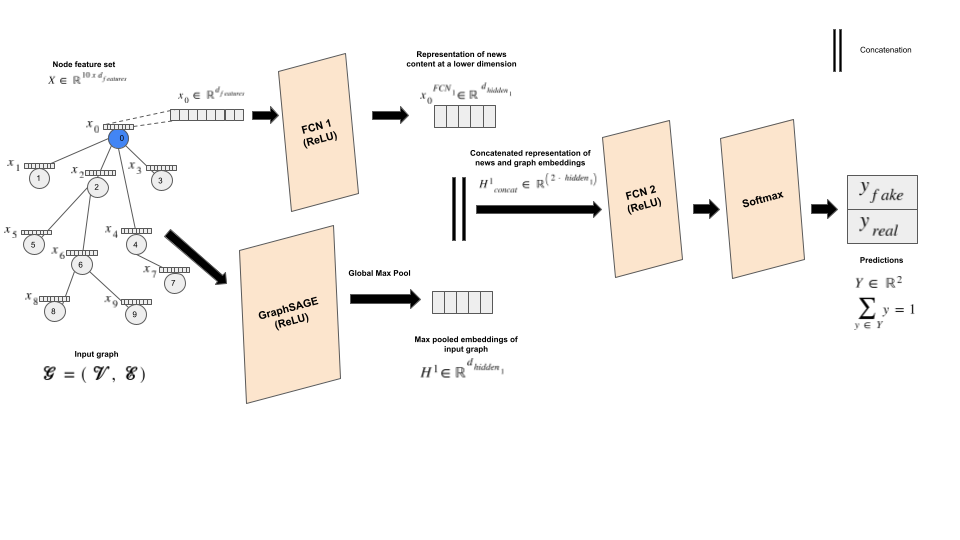
\includegraphics[scale=0.43]{UPFDClassifierArchitecture}
    \caption[UPFD classifier model pipeline]{UPFD classifer model pipeline. We used an example input graph with 10 nodes. $d_{hidden_1} = 128$ stands for hidden layer dimension of FCN 1, accordingly, $d_{hidden_2} = 2 \times d_{hidden_1} = 256$ for the hidden dimension of FCN 2, and $d_{feature} = 768$ for feature dimension.}
    \label{fig:UPFDClassifierArchitecture}
\end{figure}
We apply t-SNE~\parencite{tSNE_vanDerMaaten} using default settings provided by scikit-learn~\parencite{ScikitLearn_Pedregosa} to see if GraphSAGE is able to distinguish fake and real news before its outputs $h_v^k$ are fed to the FCN. The visualization for this procedure is provided in Fig~\ref{fig:TSNE_GraphSAGE}.
\begin{figure}
    \centering
    \subfloat[Gossipcop]{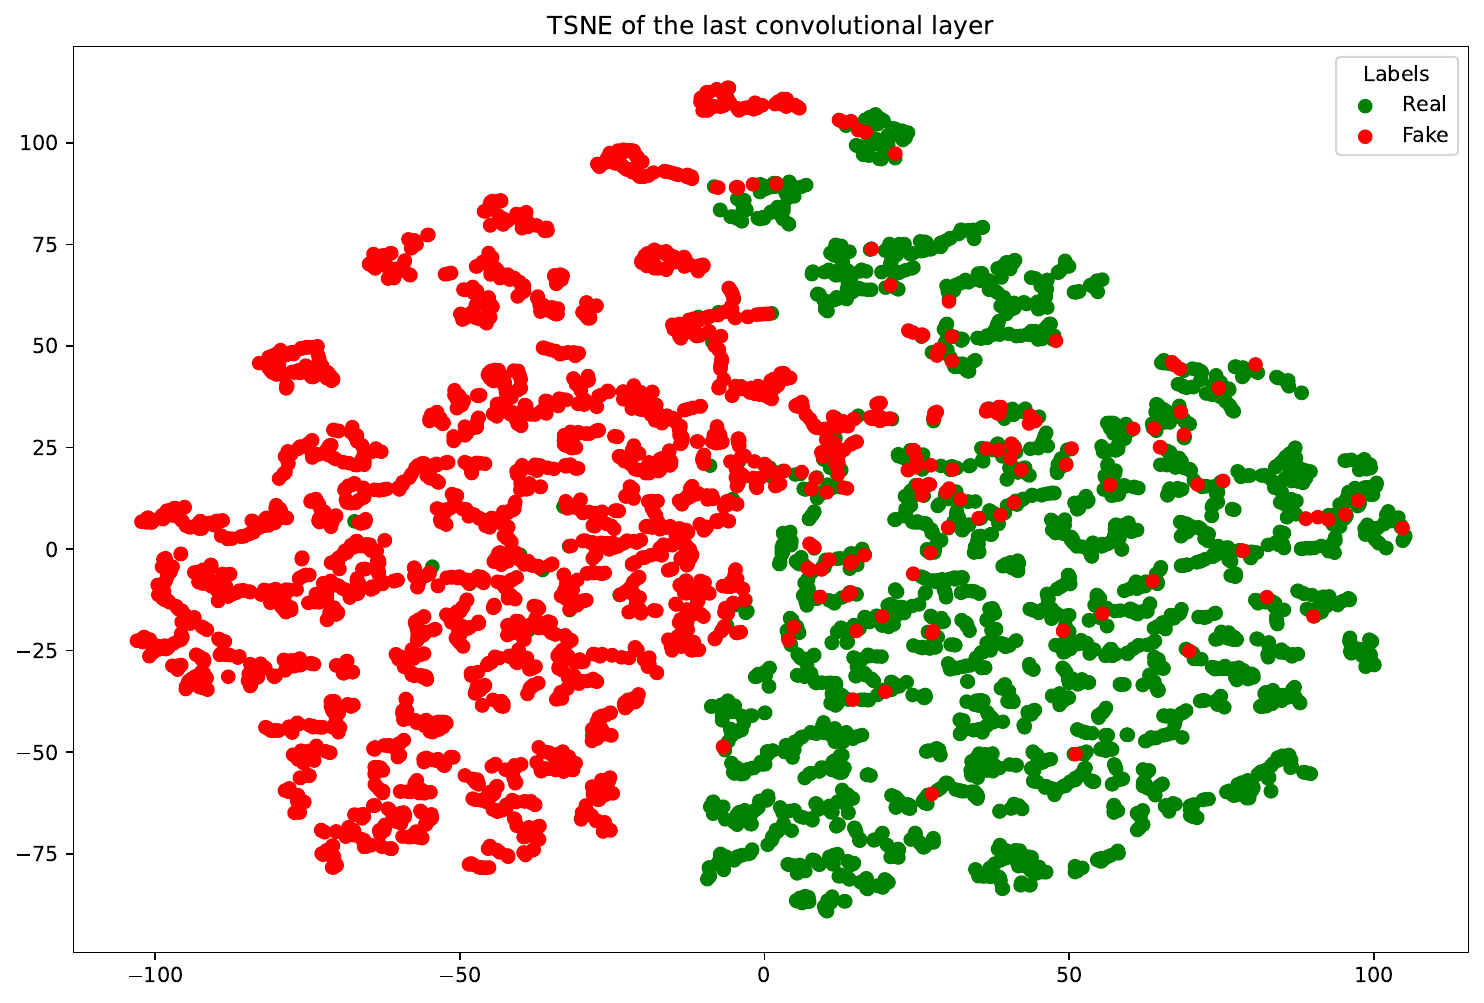
\includegraphics[width=0.45\textwidth]{TSNE_GraphSAGE_GOS.png}\label{subfig:TSNE_GraphSAGE_GOS}}
    \hfill
    \subfloat[Politifact]{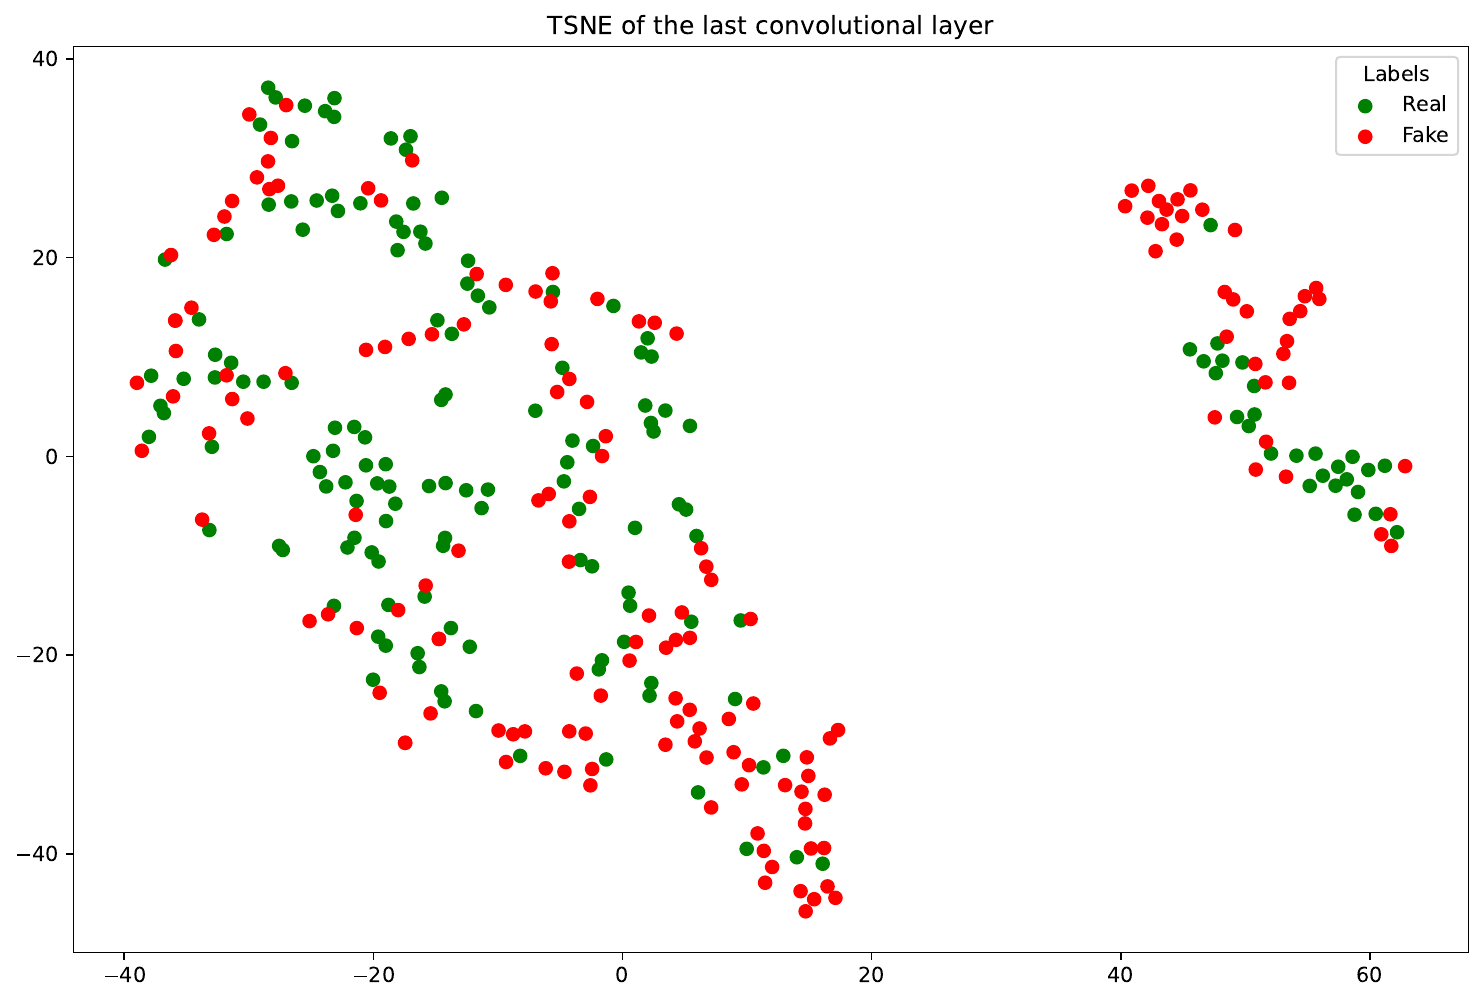
\includegraphics[width=0.45\textwidth]{TSNE_GraphSAGE_POL.png}\label{subfig:TSNE_GraphSAGE_POL}}
    \caption[t-SNE visualizations for GraphSAGE]{t-SNE visualizations for GraphSAGE on UPFD.}
    \label{fig:TSNE_GraphSAGE}
\end{figure}
Clearly GraphSAGE is able to distinguish fake and real news instances better in Gossipcop dataset, but it fails to make this discirimination with Politifact dataset. This can be due to the low amounts of instances in the Politifact dataset. After obtaining the graph encodings, the authors suggest to concatenate a representation of news content with graph embeddings. More precisely, the feature vector of root node is fed to an FCN to obtain a lower-dimensional representation which is then concatenated with graph embeddings. The concatenated vector is then fed to another FCN, and lastly the softmax layer for classification. With the setting illustrated in Fig~\ref{fig:UPFDClassifierArchitecture}, the optimizer as Adam with default $\beta_1$ and $\beta_2$, and hyperparameters provided in Table~\ref{tab:UPFDClassifier_Hyperparameters},
\begin{table}
    \centering
    \begin{tabular}{|l|l|}
        \hline
        Activation function & ReLU~\parencite{ReLU_Nair} \\
        \hline
        Batch size          & 128                        \\
        \hline
        Epochs              & 35                         \\
        \hline
        Learning rate       & 0.01                       \\
        \hline
        Hidden layer 1 size & 128                        \\
        \hline
        Hidden layer 2 size & 256                        \\
        \hline
        Weight decay        & 0.01                       \\
        \hline
    \end{tabular}
    \caption[Hyperparameters of UPFD classifier.]{Hyperparameters of UPFD classifier.}
    \label{tab:UPFDClassifier_Hyperparameters}
\end{table}
we obtain 95.49\% and 83.16\% accuracy from Gossipcop and Politifact averaged by 10 runs, respectively. All other statistics are provided in Table~\ref{tab:UPFDClassifier_Results}.
\begin{table}
    \centering
    \begin{tabular}{c | c | c | c | c}
        \textbf{Dataset} & \textbf{Accuracy} & \textbf{Precision} & \textbf{Recall} & \textbf{F1 score} \\
        \hline
        Gossipcop        & 95.49\%           & 94.95\%            & 96.17\%         & 95.50\%           \\
        \hline
        Politifact       & 83.16\%           & 84.05\%            & 82.19\%         & 83.25\%           \\
    \end{tabular}
    \caption[UPFD classifier performance metrics averaged over 10 runs.]{UPFD classifier performance metrics averaged over 10 runs.}
    \label{tab:UPFDClassifier_Results}
\end{table}

% maybe talk about the other model here

We have introduced the model we have employed for FND in mixed approaches. We will analyze the model's behavior on the graph data, and investigate its faithfulness, plausability and some other properties. We adopt GNNExplainer~\parencite{GNNExplainer_Ying} as our explanation tool and try to uncover the patterns the model have learned. We shall also discuss some limitations we encountered while conducting these experiments.

\section{GNNExplainer}
\label{sec:GNNExplainer}


